\documentclass[tikz]{standalone}

\usepackage{pgfplots}
\pgfplotsset{compat=newest}

\usepackage{tkz-tab}
\usepackage{amsmath,amssymb}

\definecolor{monbleu}{RGB}{79,106,149}
\definecolor{monrouge}{RGB}{204,67,60}
\definecolor{monvert}{RGB}{86,101,77}
\definecolor{monviolet}{RGB}{112,85,137}

\begin{document}

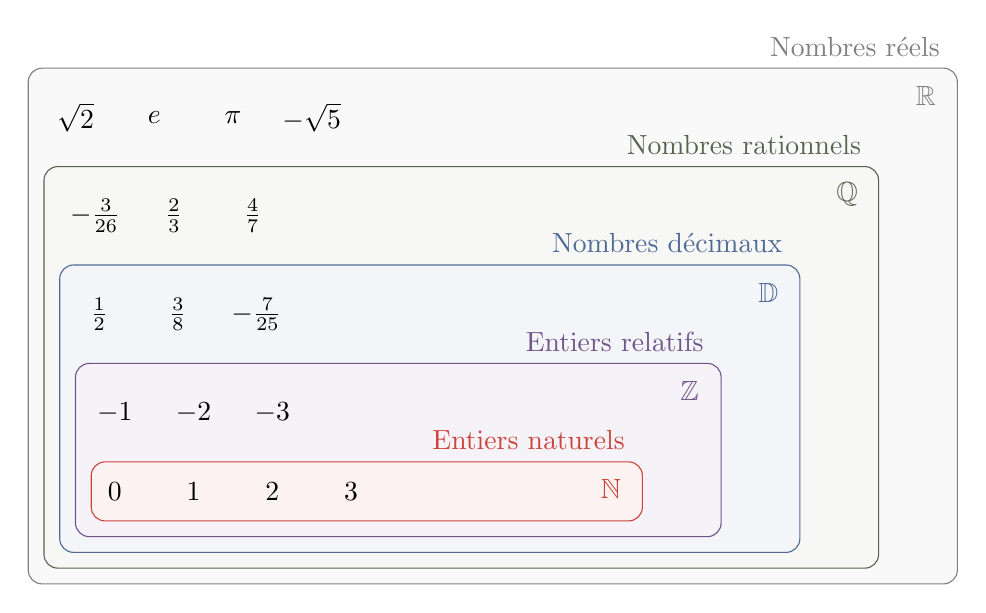
\begin{tikzpicture}
	% Ensemble R %
	\filldraw[color=gray,fill=gray!5,rounded corners=5pt] (-0.8,-0.8) rectangle (11,5.75);
	\node at (10.6,5.4) {\textcolor{gray}{$\mathbb{R}$}};
	\node[left] at (10.9,6.025) {\textcolor{gray}{Nombres réels}};
	\node at (-0.2,5.125) {$\sqrt{2}$};
	\node at (0.8,5.125) {$e$};
	\node at (1.8,5.125) {$\pi$};
	\node at (2.8,5.125) {$-\sqrt{5}$};
	% Ensemble Q %
	\filldraw[color=monvert,fill=monvert!5,rounded corners=5pt] (-0.6,-0.6) rectangle (10,4.5);
	\node at (9.6,4.15) {\textcolor{monvert}{$\mathbb{Q}$}};
	\node[left] at (9.9,4.775) {\textcolor{monvert}{Nombres rationnels}};
	\node at (0.05,3.875) {$-\frac{3}{26}$};
	\node at (1.05,3.875) {$\frac{2}{3}$};
	\node at (2.05,3.875) {$\frac{4}{7}$};
	% Ensemble D %
	\filldraw[color=monbleu,fill=monbleu!7,rounded corners=5pt] (-0.4,-0.4) rectangle (9,3.25);
	\node at (8.6,2.9) {\textcolor{monbleu}{$\mathbb{D}$}};
	\node[left] at (8.9,3.525) {\textcolor{monbleu}{Nombres décimaux}};
	\node at (0.1,2.625) {$\frac{1}{2}$};
	\node at (1.1,2.625) {$\frac{3}{8}$};
	\node at (2.1,2.625) {$-\frac{7}{25}$};
	% Ensemble Z %
	\filldraw[color=monviolet,fill=monviolet!7,rounded corners=5pt] (-0.2,-0.2) rectangle (8,2);
	\node at (7.6,1.65) {\textcolor{monviolet}{$\mathbb{Z}$}};
	\node[left] at (7.9,2.275) {\textcolor{monviolet}{Entiers relatifs}};
	\node at (0.3,1.375) {$-1$};
	\node at (1.3,1.375) {$-2$};
	\node at (2.3,1.375) {$-3$};
	% Ensemble N %
	\filldraw[color=monrouge,fill=monrouge!7,rounded corners=5pt] (0,0) rectangle (7,0.75);
	\node at (6.6,0.4) {\textcolor{monrouge}{$\mathbb{N}$}};
	\node[left] at (6.9,1.025) {\textcolor{monrouge}{Entiers naturels}};
	\node at (0.3,0.375) {$0$};
	\node at (1.3,0.375) {$1$};
	\node at (2.3,0.375) {$2$};
	\node at (3.3,0.375) {$3$};
\end{tikzpicture}

\end{document}